\apendice{Documentación técnica de programación}

\section{Introducción}
En este anexo, se describe la estructura del proyecto en directorios, la instalación del mismo y el proceso que se ha llevado a cabo para poder desplegarlo con Heroku.
\section{Estructura de directorios}
Se detalla a continuación la estructura que tiene el proyecto en en la organización de su código fuente, estando todo ello disponible en GitHub, excepto ciertos archivos que contienen información confidencial.
El directorio raíz \textit{'main'} se descompone en:
\begin{itemize}
    \item \textit{/Code:}\\
    Contiene los archivos \textit{.py} a los que llama la función principal \textit{'main'} para realizar todas las operaciones que necesite:
    \begin{itemize}
        \item Busqueda\_XacoMeterII.py:\\
        Contiene el diccionario desde el que se realizan las búsquedas con la API de Twitter.
        \item CrearTablasBD\_XacoMeterII.py:\\
        Contiene cada una de las operaciones que se van a realizar en la base de datos (UPDATE, SELECT...)
        \item Destinos\_XacoMeterII.py:\\
        Operaciones que realizan las llamadas a los archivos \textit{.py} que solicitan los datos a la API de Twitter y almacena la información en la base de datos.
        \item FunciónPrincipal\_XacoMeterII.py:\\
        Realiza la conexión con la API de Twitter y solicita la información requerida.
        \item GraficosEstadisticas\_XacoMeterII.py:\\
        Crea los gráficos, con la herramienta \textit{"Plotly"} de las estadísticas de los datos almacenados en la base de datos.
        \textit{"SentimentAnalysis\_XacoMeterII.py:}\\
        Realiza el cálculo del índice de sentimiento de los tweets almacenados de cada BIC.
    \end{itemize}
    \item \textit{/data:}\\
    Contiene los datos en formato csv.
    \begin{itemize}
        \item inventario\_01.csv:\\
        Este csv contiene todos los datos de los BICs según la organización que lleva la Junta de Castilla y León.
    \end{itemize}
    \item \textit{/static:}\\
    Contiene el archivo \textit{styles.css} el cual contiene contiene los estilos que se van a aplicar en la página web y las imágenes que se van a utilizar para mostrar en cada una de las páginas de la aplicación, por ejemplo, el logo de XacoMeterII.
    \item \textit{/templates:}\\
    Contiene todos los archivos \textit{.html} que definen la parte visual de la aplicación.
    \begin{itemize}
        \item admin\_Actualizar.html
        \item admin\_Crear.html
        \item administradorOpciones.html
        \item barraLateral.html
        \item base2.html
        \item home.html
        \item login.html
        \item serieTemporal.html
    \end{itemize}
    \item \textit{/venv:}\\
    Contiene un árbol de directorios con ejecutables en Python que indican que es un entorno virtual.
    \item \textit{.gitignore:}\\
    Fichero que contiene el nombre de los archivos ocultos para GitHub.
    \item \textit{.env:}\\
    Fichero sensible con las contraseñas necesarias para el desarrollo del proyecto. Este archivo estará oculto para GitHub.
    \item \textit{LICENSE:}\\
    Licencia de la aplicación
    \item \textit{errores.log:}\\
    Archivo en el que se guardan los errores generados por la aplicación web ejecutada en local durante su uso.
    \item \textit{Procfile:}\\
    Archivo que especifica cuál es el archivo principal de la aplicación para Heroku.
    \item \textit{README.md:}\\
    Archivo que contiene una breve descripción del proyecto y unos primeros pasos para su utilización.
    \item \textit{ejecutable.bat:}\\
    Archivo \textit{batch} que ejecuta los comandos necesarios para activar el entorno y ejecutar la aplicación web con el fin de no tener que usar Visual Code y poder ver la aplicación local en el navegador.
    \item \textit{main.py:}\\
    Archivo Python principal que realiza las llamadas a los demás archivos.
    \item \textit{requirements.txt:}\\
    Archivo que contiene un listado de las herramientas utilizadas -con sus versiones- para realizar el despliegue en Heroku.
    
\end{itemize}


\section{Manual del programador}
En este apartado se va a proceder a explicar los progrmas utilizados, su instalación y la razón de su uso.\\
El proyecto ha sido desarrollado de manera local en el equipo, se ha desplegado en Heroku y para la realización de pruebas en modo Administrador se dispondrá de una maquina virtual simulando el equipo local.\\
\subsection{Visual Studio Code}
Visual Studio Code se utiliza para realizar el desarrollo de la aplicación, la creación de archivos y métodos para el funcionamiento del proyecto.
Para la descarga de Visual Studio Code entramos en la página web \url{https://code.visualstudio.com/download} y seleccionamos, en nuestro caso, la versión para Windows (Figura D.1).\\
\begin{figure}[h!]
    \centering
    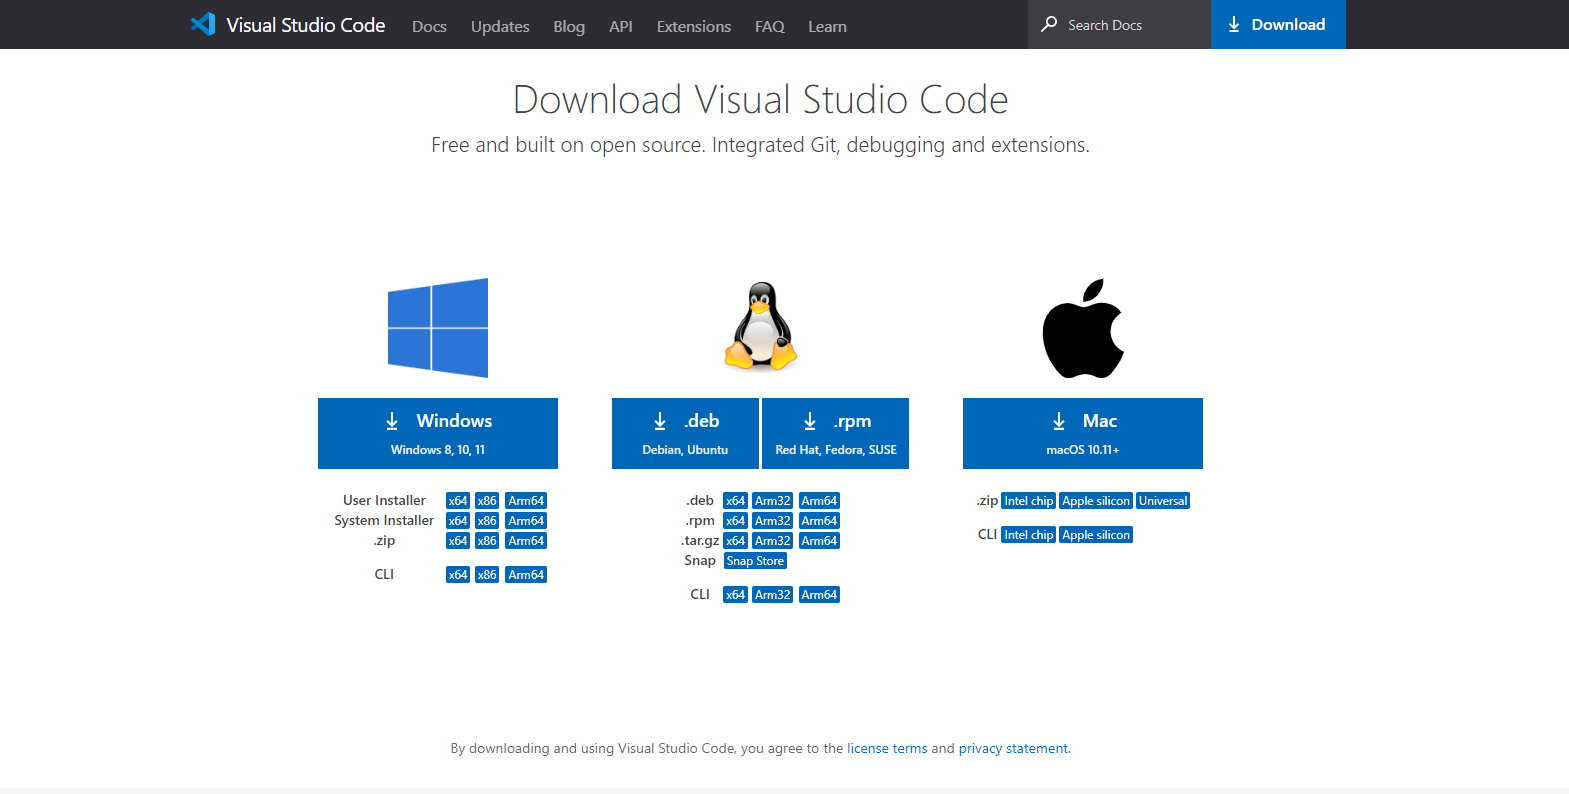
\includegraphics[scale=0.3]{img/VisualCode.png} \\
    \caption{Documentación del programador - Visual Studio Code}
    \label{Documentación del programador - Visual Studio Code}
\end{figure}
Una vez descargada la aplicación, debemos abrir el archivo de instalación \textit{.exe} para instalarlo y seguir los pasos hasta leer y aceptar el acuerdo de la licencia.
Una vez realizados los anteriores pasos, ya es posible empezar a trabajar con Visual Studio Code.
\subsection{PostgreSQL}
PostgreSQL es la base de datos que se ha decidido utilizar para la gestión de la base de datos, ya que puede ser desplegada en Heroku.\\
Para su descarga debemos entrar en la página \url{https://www.postgresql.org/download/} y pulsar sobre el icono de Windows. Una vez seleccionado Windows, debemos seleccionar la versión. Lo recomendable es utilizar la última versión, ya que siempre será la más actualizada, en este caso la versión 15 para Windows de 64-bit (Figura D.2). 
\begin{figure}[h!]
    \centering
    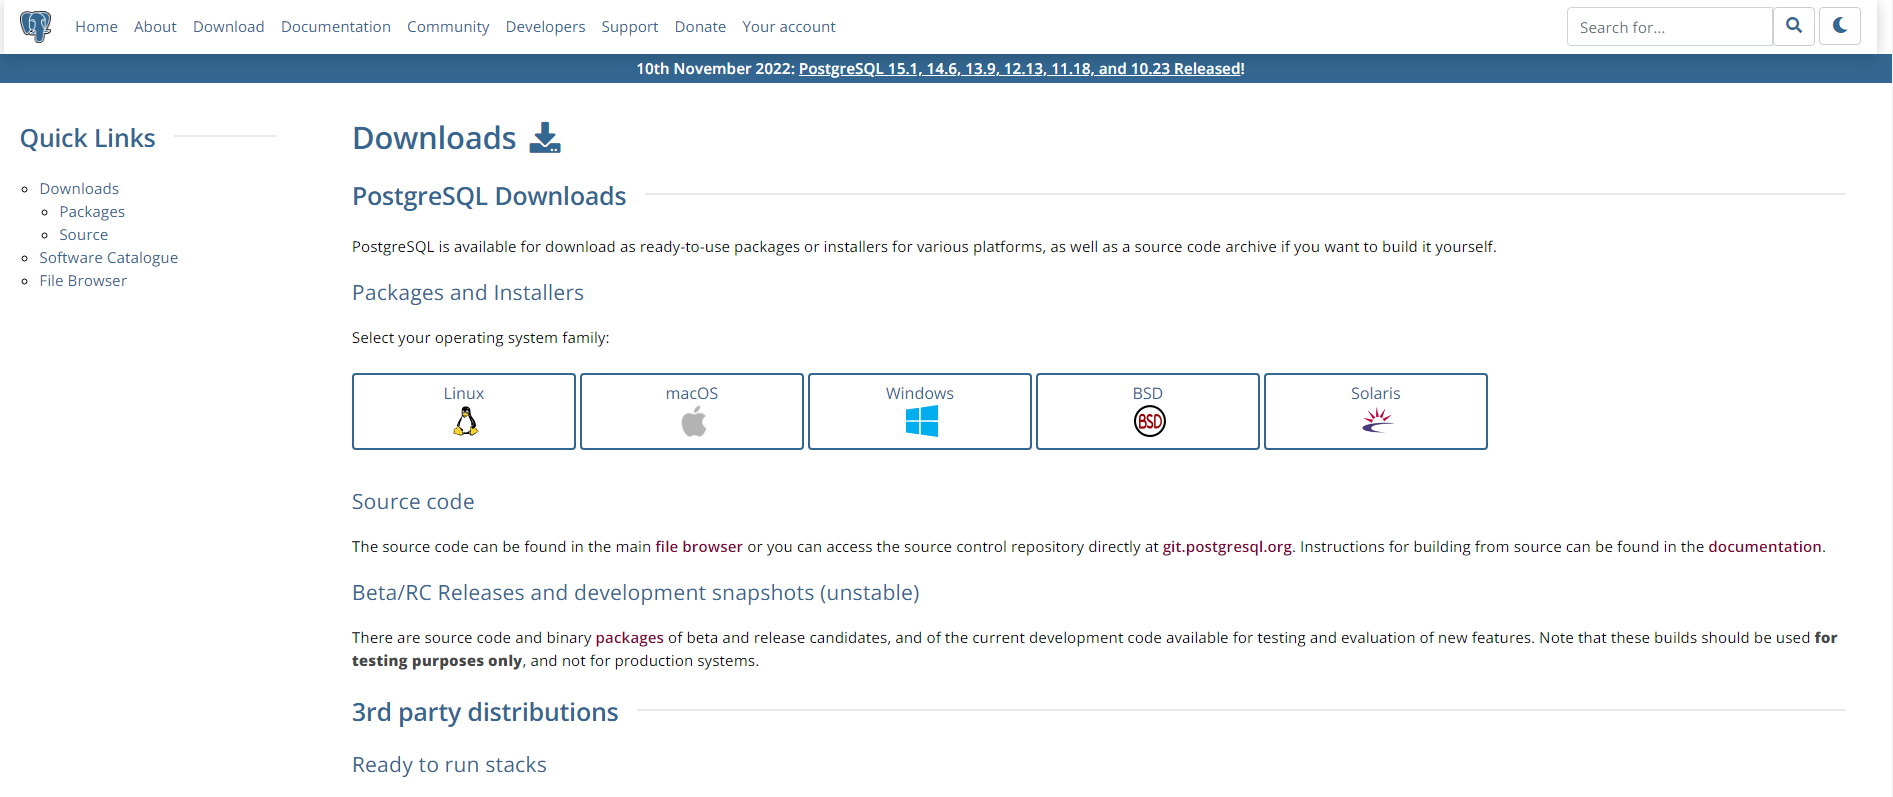
\includegraphics[scale=0.2]{img/postgreSQL.png}\\
    \caption{Documentación del programador - PostgreSQL}
    \label{Documentación del programador - PostgreSQL}
\end{figure}

Una vez que ha sido descargada, debemos busar el archivo \textit{.exe} y ejecutarlo para realizar la instalación.\\
Solamente se necesita continuar con todos los pasos y aceptar la licencia de PostreSQL.\\
Una vez tengamos todo instalado, hay que configurarlo para poder acceder a la base de datos de Heroku.\\
Para ello, creamos un nuevo servidor (Figura D.3):
\begin{figure}[h!]
    \centering
    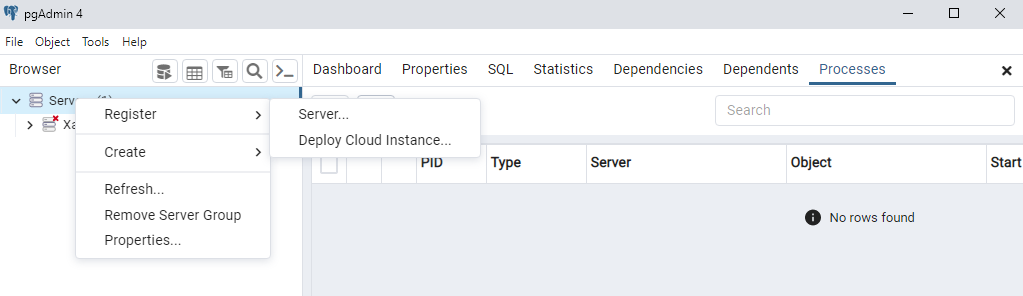
\includegraphics[scale=0.5]{img/nuevoServer.png}
    \caption{Documentación del programador - Crear servidor}
    \label{Documentación del programador - Crear servidor}
\end{figure}


Y realizamos la configuración con los datos que obtenemos del Add-on de Heroku (Figura D.4, Figura D.5, Figura D.6):\\
\begin{figure}[H]
    \hspace{0.2cm}
    \begin{minipage}[b]{0.3\linewidth}
        \centering
        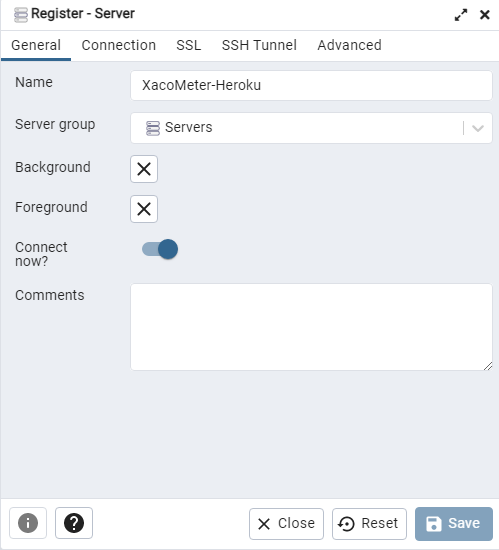
\includegraphics[scale=0.3]{img/GeneralPostgresql.png} \\
        \caption{Documentación del programador - pgAdmin4 general}
        \label{Documentación del programador - pgAdmin4 general}
    \end{minipage}
    \hspace{0.2cm}
    \begin{minipage}[b]{0.3\linewidth}
        \centering
        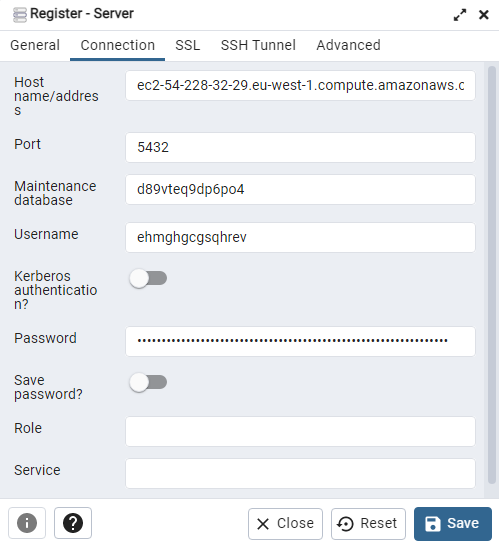
\includegraphics[scale=0.3]{ConnectionPostgresql.png}
        \caption{Documentación del programador - pgAdmin4 conexión}
        \label{Documentación del programador - pgAdmin4 conexión}
    \end{minipage}
    \hspace{0.2cm}
    \begin{minipage}[b]{0.3\linewidth}
        \centering
        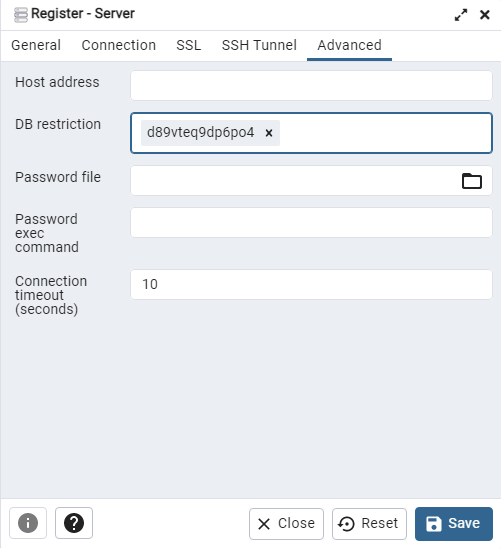
\includegraphics[scale=0.3]{AdvancedPostgresql.png}
        \caption{Documentación del programador - pgAdmin4 avanzado}
        \label{Documentación del programador - pgAdmin4 avanzado}
    \end{minipage}
\end{figure}
\subsection{Virtual Box}
En el caso de este proyecto vamos a elegir una máquina virtual para poder exportar el proyecto y que se puedan realizar pruebas en local del mismo, pudiendo así utilizar la función de Administrador, que por las limitaciones de Heroku, no permiten comprobar su funcionamiento.\\ Yo he decidido usar “VirtualBox” porque frente a otras
plataformas, como puede ser VMware, la interfaz de usuario es muy sencilla y además tiene
un mejor rendimiento, por lo que es más rápida y podemos utilizar las \textit{“guest additions”}
como tener carpetas compartidas con nuestro equipo o arrastrar y copiar del
portapapeles respecto al equipo anfitrión.\\
\begin{enumerate}
    \item \textbf{Instalación de VirtualBox:}
    Nos dirigimos a \url{www.virtualbox.org}, entramos en descargas y seleccionamos la versión
    que queremos y el paquete indicado para nuestro sistema operativo, Windows hosts (Figura D.7).
    Para instalarlo solo debemos seguir los pasos que se nos indican y al terminar pulsar el
    botón “FINISH”.
    \begin{figure}[h!]
        \centering
        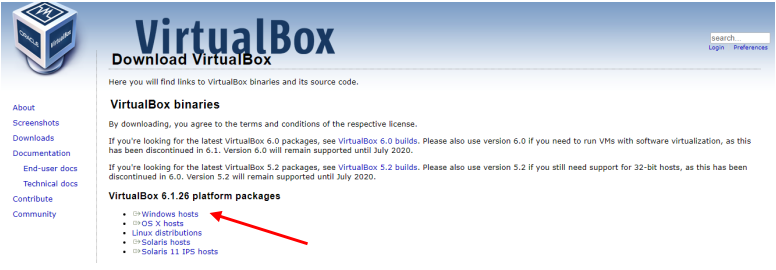
\includegraphics[scale=0.6]{img/DescargaVirtualBox.png} \\
        \caption{Documentación del programador - VirtualBox}
        \label{Documentación del programador - VirtualBox}
    \end{figure}
    \item \textbf{Instalación del sistema operativo:}
    En este caso, se va a utilizar Windows 10 Pro, con una licencia OEM que se ha comprado a través de RoyalCDKeys.\cite{RoyalCDKeys}\\
    Entramos en la página \url{https://www.microsoft.com/es-es/software-download/windows10} y, para poder decargar la ISO, solo hace falta dar a la tecla F12 para navegar como un desarrollador y elegir la última versión, ya que es la más actualizada, de Windows 10 de 64 bits y dar al botón descargar.\\
    Creamos una máquina dentro de VirtualBox pulsando en el botón de “nueva”. Ponemos el
    nombre que queremos para nuestra máquina virtual, en este caso XacoMeter\_NataliaFranco, y el sistema operativo que hemos decidido que vamos a instalar (Windows 10 64-bit). Le damos al botón \textit{Next} y nos dice que le indiquemos cuánta RAM queremos que tenga; este valor es mejor dejarlo como
    se nos recomienda, ya que si lo ampliamos, nos quitaría memoria de nuestro sistema
    operativo anfitrión (Windows). A continuación, creamos un disco duro VDI para almacenar el sistema
    operativo que le vamos a introducir y también, los archivos y programas (aproximadamente 25Gb
    es una cifra suficiente para trabajar con la máquina perfectamente).\\
    Para instalar Windows 10 en la máquina que hemos creado, vamos al botón de
    “Configuración”, a “Almacenamiento” y en “Controlador: IDE” añadimos una unidad
    óptica. Seleccionamos el archivo ISO que tenemos descargado y aceptamos (Figura D.8).
    \begin{figure}[h!]
        \centering
        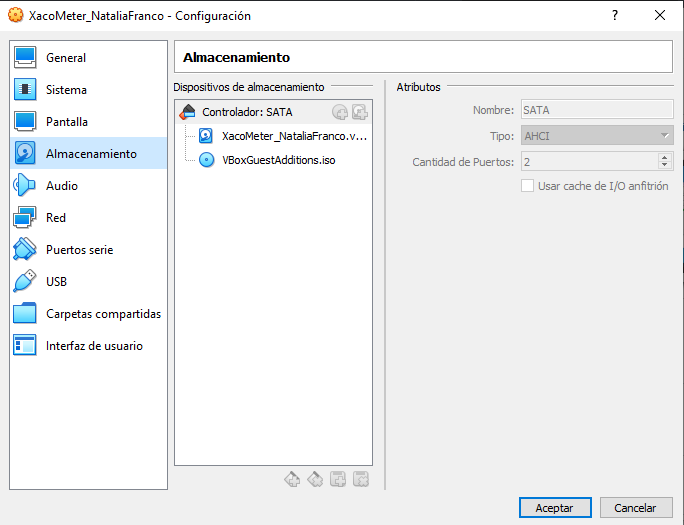
\includegraphics[scale=0.7]{img/ISO.png} \\
        \caption{Documentación del programador - Windows 10}
        \label{Documentación del programador - Windows 10}
    \end{figure}

    
    Al abrir la máquina nos aparecerá la instalación de Windows, introducimos la licencia que hemos comprado de Windows 10 Pro OEM y aceptamos los términos de la licencia.
    \item \textbf{Instalación de programas:}
    Una vez realizada la instalación, se deben seguir los pasos anteriormente descritos para la instalación de Visual Studio Code y pgAdmin4.\\
    Se importan los archivos a la máquina virtual para su uso y se configura la base de datos.\\
    Además, se descargará Google Chrome, donde se podrá ver la aplicación web y probarla.
    \item \textbf{Exportación de máquina virtual:}
    En VirtualBox, pulsar sobre "Archivo" y "Exportar servicio virtualizado". Solo hay que indicar la máquina virtual a exportar y el nombre con la extensión, en este caso, \textit{XacoMeter\_NataliaFranco.ova}.
\end{enumerate}
\section{Compilación, instalación y ejecución del proyecto}
La ejecución del proyecto se puede realizar de dos maneras, en función de las utilidades que se le vayan a dar. El proyecto puede ejecutarse bien en local, a través de la máquina virtual que se facilita o bien, a través de la página web desplegada en heroku.
\subsection{Ejecución en local}
Para la ejecución del proyecto en local, se facilita una máquina virtual de VirtualBox con el sistema operativo Windows 10 con Visual Studio Code y PostgreSQL instalado para la comodidad de los usuarios administradores.\\
Esta máquina se facilita ya que, debido a las restricciones de la API de Twitter y el tiempo de ejecución de ciertas operaciones del modo administrador, no podrán ser utilizadas en la página desplegada ya que se recibirá un \textit{timeout.}\\
El pin del usuario XacoMeter en Windows es: '1761'\\
Una vez se haya ingresado en la cuenta se debe abrir la aplicación de Visual Studio Code e introducir los siguientes comandos (Figura D.9):\\
\begin{itemize}
    \item Activar el entorno virtual: \\
    \textit{.venv\textbackslash{Scripts\textbackslash{activate}}}
    \item Compilar el proyecto:\\
    \textit{python main.py}
\end{itemize}
\begin{figure}[h!]
    \centering
    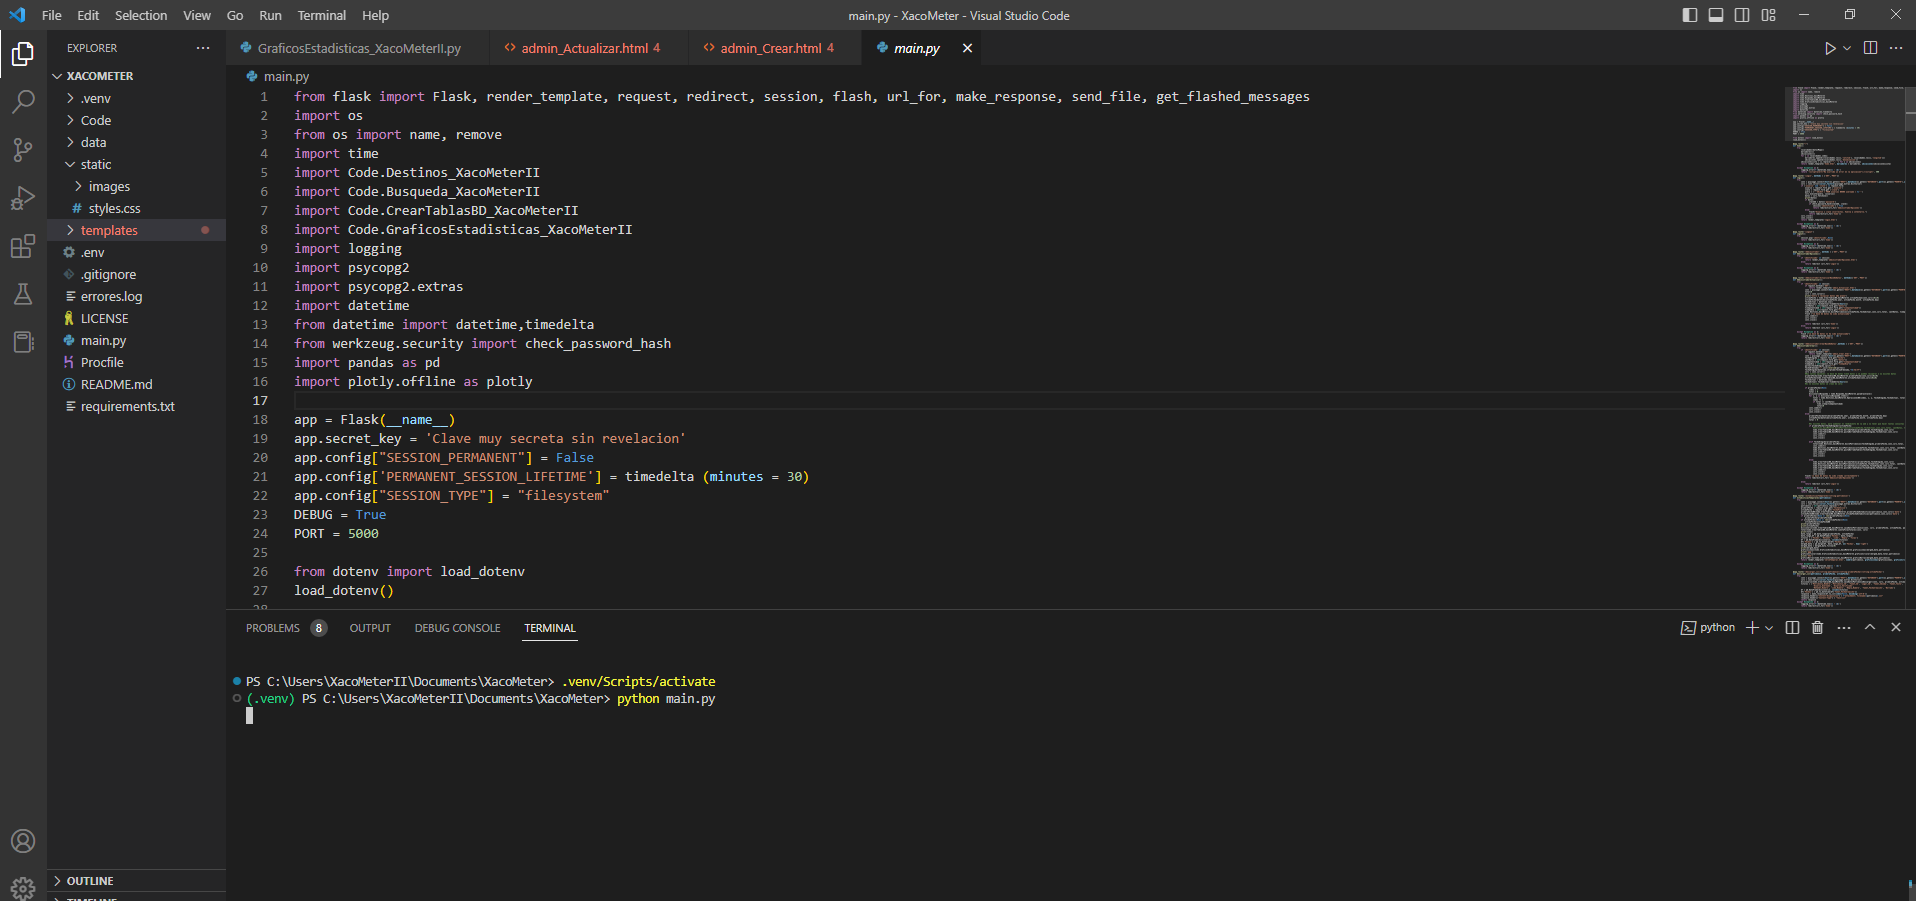
\includegraphics[scale=0.25]{img/Ejecutar.png} \\
    \caption{Documentación del programador - Comandos VS}
    \label{Documentación del programador - Comandos VS}
\end{figure}
También se ofrece la opción del uso del archivo \textit{ejecutable.bat}. Este es un archivo \textit{batch}, el cual, al hacer click sobre él, ejecuta los comandos que activan el entorno virtual y ejecutan el proyecto, lo cual permite que no se necesite abrir Visual Studio Code ni ejecutar comandos. Se ha creado un acceso directo en el escritorio de la máquina virtual del mismo para una mayor comodidad.\\

Para abrir la aplicación web se debe acceder desde el navegador (está instalado en la máquina virtual Microsoft Edge) a la URL \url{http://127.0.0.1:5000}.\\
Si se quieren visualizar las tablas de la base de datos, se necesita entrar en pgAdmin4 con el usuario: 'postgres' y la contraseña 'postgres'. Entrando en el servidor XacoMeter-Heroku, en la base de datos "d89vteq9dp6po4" con la contraseña "7b3278563bc4d86a321b8aab5716ef7b2e760978dfb4a23d8a392b36ea94d081" se podrán ejecutar las consultas deseadas con sql o ver las tablas en Schemas>public>Tables (Figura D.10).
\begin{figure}[h!]
        \centering
        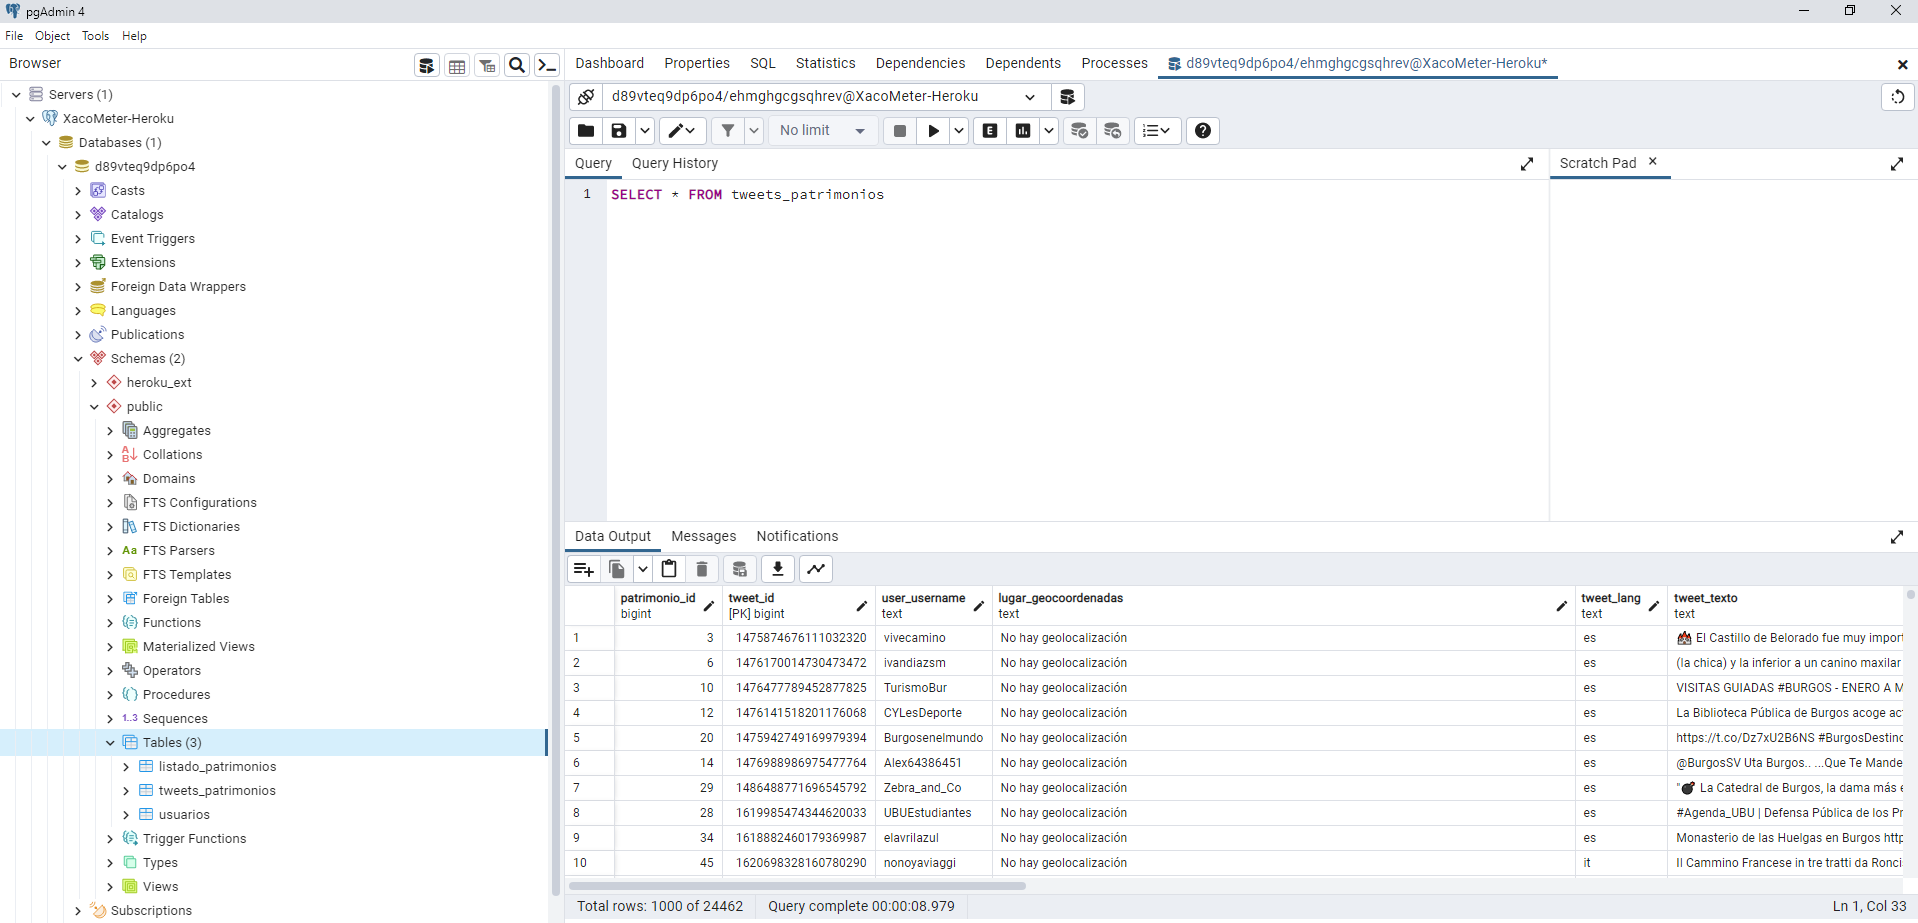
\includegraphics[scale=0.25]{img/pgAdmin4.png} \\
        \caption{Documentación del programador - pgAdmin 4}
        \label{Documentación del programador -pgAdmin 4}
    \end{figure}
\subsection{Despliegue en Heroku}
Para desplegar la aplicación en Heroku, al ser de pago, se debe conectar nuestra cuenta de GitHub con Heroku, ya que de esta manera, al ser estudiante, Heroku te permite obtener una cuantía de créditos suficientes para el despliegue del proyecto durante varios meses.\\
Deberemos crear una aplicación en Heroku indicando el nombre y la región de la aplicación que va a ser utilizada para localizar la página web (Figura D.11).
\begin{figure}[h!]
    \centering
    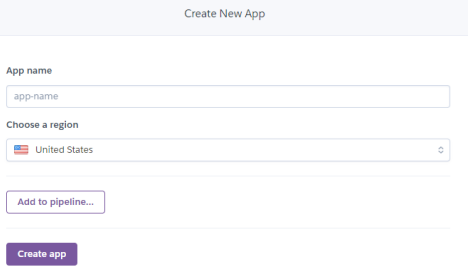
\includegraphics[scale=0.6]{img/CrearAPP.png} \\
    \caption{Documentación del programador - Heroku App}
    \label{Documentación del programador - Heroku App}
\end{figure}


Para el despliegue de la aplicación en Heroku, se necesita tener un archivo \textit{Procfile} que indique el comando a ejecutar en Heroku con el archivo principal, y también un archivo \textit{requirements} que contenga el nombre y la versión de todas las librerias necesarias para la ejecución del proyecto.\\
Para el despliegue de la base de datos en Heroku, se necesita activar un \textit{Add-On} de Heroku PostgreSQL (Figura D.12), que crea una base de datos en la nube con un usuario, una contraseña que te facilita Heroku.
\begin{figure}[h!]
    \centering
    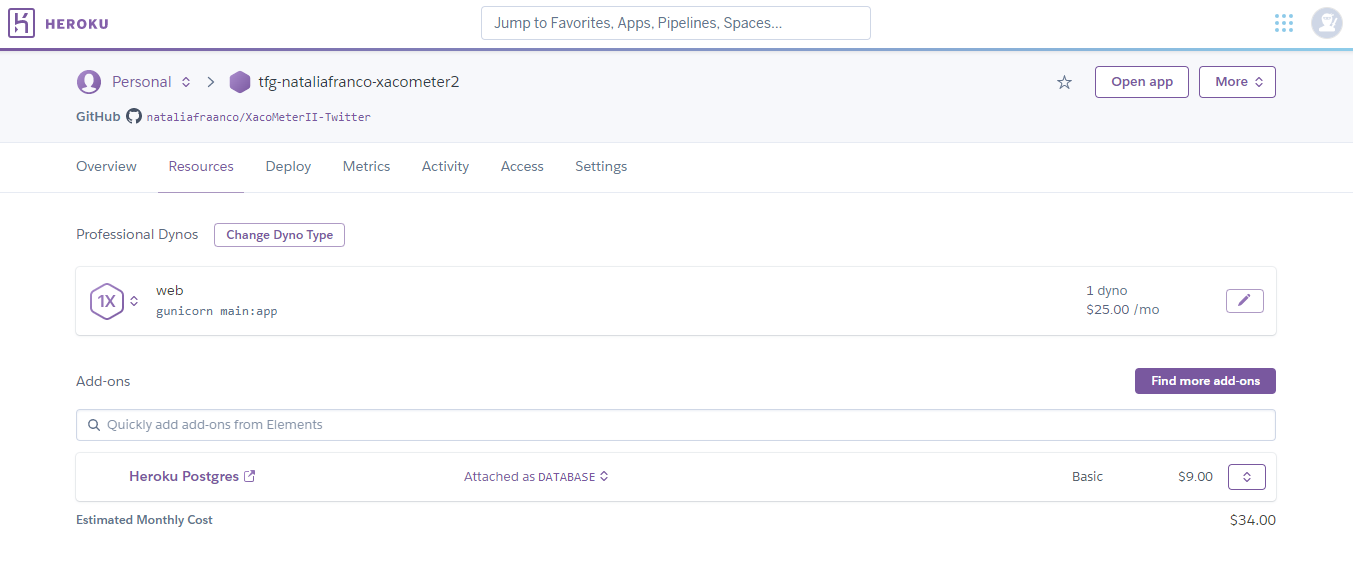
\includegraphics[scale=0.3]{img/Resources.png} \\
    \caption{Documentación del programador - Recursos}
    \label{Documentación del programador - Recursos}
\end{figure}


Para realizar el cambio de la base de datos local a la base de datos desplegada, tan solo se necesitará crear un \textit{backup}, o copia de seguridad, de la base de datos local y cargarla en la base de datos nueva de Heroku. Además, en el proyecto, para que se utilice la nueva base de datos desplegada, tan solo hará falta cambiar los parámetros de la base de datos en las variables de entorno guardadas en el archivo \textit{.env}.


Heroku, despliega la aplicación desde los archivos guardados en tu GitHub. En nuestro caso, como hay archivos como \textit{.env} que contienen información confidencial, como las contraseñas, estos no deben subirse a GitHub y deberán configurarse directamente en las variables de entorno de Heroku (Figura D.13):\\
\begin{figure}[h!]
    \centering
    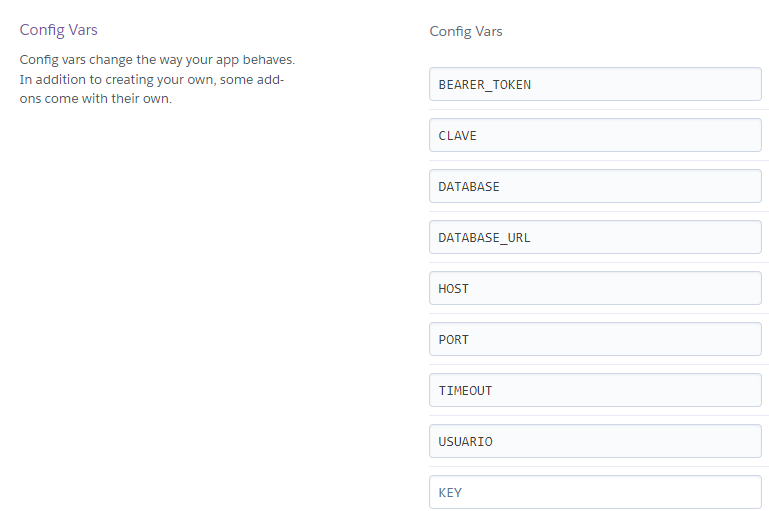
\includegraphics[scale=0.5]{img/ConfigVars.png} \\
    \caption{Documentación del programador - Configuración de variables}
    \label{Documentación del programador - Configuración de variables}
\end{figure}


Una vez hayamos configurado todo lo anterior, ya podremos desplegar el proyecto pulsando sobre \textit{'Deploy Branch'} (Figura D.14).
\begin{figure}[h!]
    \centering
    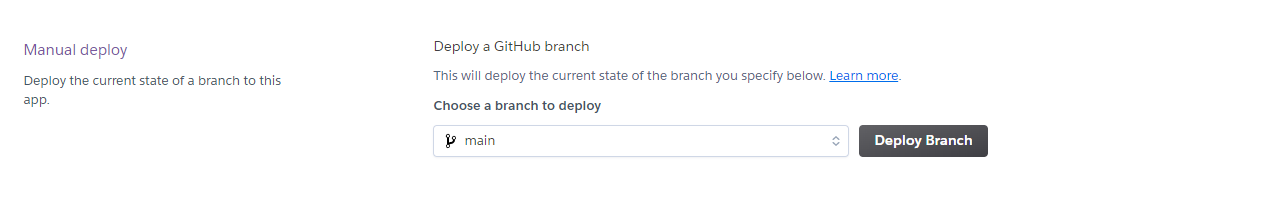
\includegraphics[scale=0.5]{img/DeployBranch.png} \\
    \caption{Documentación del programador - Desplegar rama}
    \label{Documentación del programador - Desplegar rama}
\end{figure}
\section{Pruebas del sistema}
Como pruebas de la aplicación XacoMeterII, cabe destacar que se han realizado las siguientes:
\begin{enumerate}
    \item Comprobar que con los parámetros introducidos por defecto, la API de Twitter no deniega la generación de información.
    \item Poner decimales a los valores de los parámetros que deben ser enteros, no debe permitirlo.
    \item Probar el modo administrador con parámetros no permitidos para la API de Twitter.
    \item No introducir fecha de inicio en la creación de la base de datos.
    \item Introducir mal el usuario y contraseña del administrador para comprobar que no permite acceder.
    \item Introducir desde la URL las direcciones de actualizar y crear la base de datos para comprobar el correcto funcionamiento de denegar el acceso y redireccionar a la página de inicio de sesión.
    \item Comprobar que funcionan todas las redirecciones de los BICs en el inicio, tanto con el uso del mapa como del desplegable.
    \item Introducir en la página de estadísticas una fecha mayor de inicio que la fecha final, la aplicación debe mostrar que no hay datos entre esas fechas ya que siempre debe ser menor la fecha de inicio.
    \item Probar la funcionalidad de descarga del csv y que la importación en Excel puede realizarse correctamente mostrando todos los parámetros.
    \item Probar el funcionamiento de la barra navegadora.
    \item Probar el análisis de sentimientos.
    \item Introducir errores para visualizar mensajes de error.

\end{enumerate}